\chapter{Sviluppi tecnologici}\label{ch:sviluppi}
Questo capitolo riguarda gli sviluppi realizzati dal punto di vista tecnologico che sono andati direttamente ad impattare la piattaforma AirQino, migliorandone in un caso l'affidabilità dei dati e nell'altro i tempi di risposta del database per query particolarmente onerose.

% Replica del database di produzione
\section{Replica del database di produzione}\label{sec:replica}

Spesso fare analisi mediamente complesse sui dati contenuti in un database può comportare rallentamenti nei tempi di risposta. Se questi carichi risultano frequenti, il sistema può arrivare a bloccarsi e provocare interruzioni del servizio. Una soluzione per risolvere questo problema è la creazione di una (o più) \textbf{repliche} del database primario. Nella replica, i dati e gli oggetti del database vengono copiati e distribuiti su un altro spazio fisico. Le operazioni onerose a questo punto possono essere fatte direttamente sulla replica che agisce come nodo secondario: in questo modo, il carico viene distribuito e non si intaccano le performance del database principale.

Il concetto di \textit{replica} è diverso dal \textit{mirroring}, in cui vengono create una o più copie di un database su diverse istanze del server, e funzionano come copie di riserva (e si attivano soltanto nel caso di guasto del nodo principale).

Un sistema di replica correttamente implementato può offrire diversi vantaggi, tra cui \textbf{riduzione del carico} (perchè i dati replicati possono essere distribuiti su più server), \textbf{efficienza} (i server offrono prestazioni migliori perchè meno gravati da query pesanti) e \textbf{ridondanza} (i dati sono raggiungibili da più indirizzi).

Di contro, questa tecnica comporta la necessità di mantenimento dei nodi secondari, spesso collocati su server diversi (con i costi a questi associati). Inoltre, repliche errate o non implementate in maniera corretta possono causare la mancata sincronizzazione tra i nodi, portando ad una perdita o incoerenza dei dati.

\subsection{Motivazioni}\label{ssec:replica-motivazioni}
L'affidabilità dei dati rappresenta uno dei punti critici per un sistema di ingestione di grosse quantità di dati. Questo è vero anche caso di AirQino, dove il database di produzione conta oltre 100 milioni di misurazioni rilevate, in continuo aumento, con una media di 300 inserimenti al minuto. In questo scenario la replicazione dei dati può portare diversi vantaggi, principalmente legati alle prestazioni, disponibilità e sicurezza dei dati:
\begin{enumerate}
  \item \textbf{Maggiore affidabilità}: tramite la replica del database viene garantita la disponibilità dei dati anche nel caso in cui una delle macchine presenti un guasto hardware;
  \item \textbf{Miglioramento delle prestazioni}: essendo i dati distribuiti su diverse istanze, accessi multipli non saturano i server. Questo aspetto risulta particolarmente importante per applicazioni con una grande quantità di richieste simultanee;
  \item \textbf{Maggiore sicurezza dei dati}: Mentre in un sistema tradizionale i backup di un database (se effettuati) sono archiviati sullo stesso disco, con la replica del database possono essere distribuiti su più server, aumentandone di fatto l'affidabilità e la ridondanza.
\end{enumerate}

Esistono diverse tecniche di replicazione del database, che dipendono sia dalla tecnologia utilizzata (MySQL \cite{mysql}, Postgres \cite{postgres}) che dalla natura del database stesso (relazionale o non relazionale). Il database di AirQino fa uso di \textbf{Timescale} \cite{timescale}, un database relazionale open source per la gestione efficienti di dati temporali basato su Postgres; una caratteristica di Postgres è proprio la possibilità di replicazione tramite l'utilizzo della tecnologia di \textbf{streaming replication}, descritta di seguito.

\subsection{Streaming replication}\label{ssec:streaming-replication}
La \textit{streaming replication} è una funzionalità che consente di replicare i dati in tempo reale da una istanza di database Postgres a un'altra. Questo significa che se si modificano i dati in una delle istanze, questi saranno immediatamente replicati anche nelle altre. Questa replica di lettura (\textit{standby} in termini Postgres) è di fatto una copia fisica creata in modo asincrono dell'istanza del database primario.

Postgres fa uso di un ruolo speciale detto di replica (\textit{replication role}) per eseguire la replica in streaming. Questo presenta dei privilegi ma non può essere utilizzato per modificare i dati: la replica infatti è di \textbf{sola lettura}.

La gestione della replicazione si basa sulle transazioni \textbf{WAL} (\textit{Write Ahead Log}) e utilizza il protocollo TCP per garantire una connessione sicura tra i server, e inviare in modo asincrono le modifiche al database via via che vengono effettuate. Postgres salva le informazioni aggiornate del server primario in registro delle transazioni, noto come registro \textit{write-ahead}, utile anche in fase di preparazione per il ripristino dopo un'interruzione o per un \textit{rollback}. La replica in streaming funziona proprio trasferendo e applicando il registro al server di replica in tempo reale (figura \ref{fig:streaming-replication}).

È possibile anche promuovere una replica di lettura Postgres a una nuova istanza database di origine. Una volta promossa, la replica smette di ricevere comunicazioni WAL e non è più un'istanza di sola lettura, ma agisce di fatto come nodo primario.

\begin{figure}[H]
\centering
\captionsetup{justification=centering}
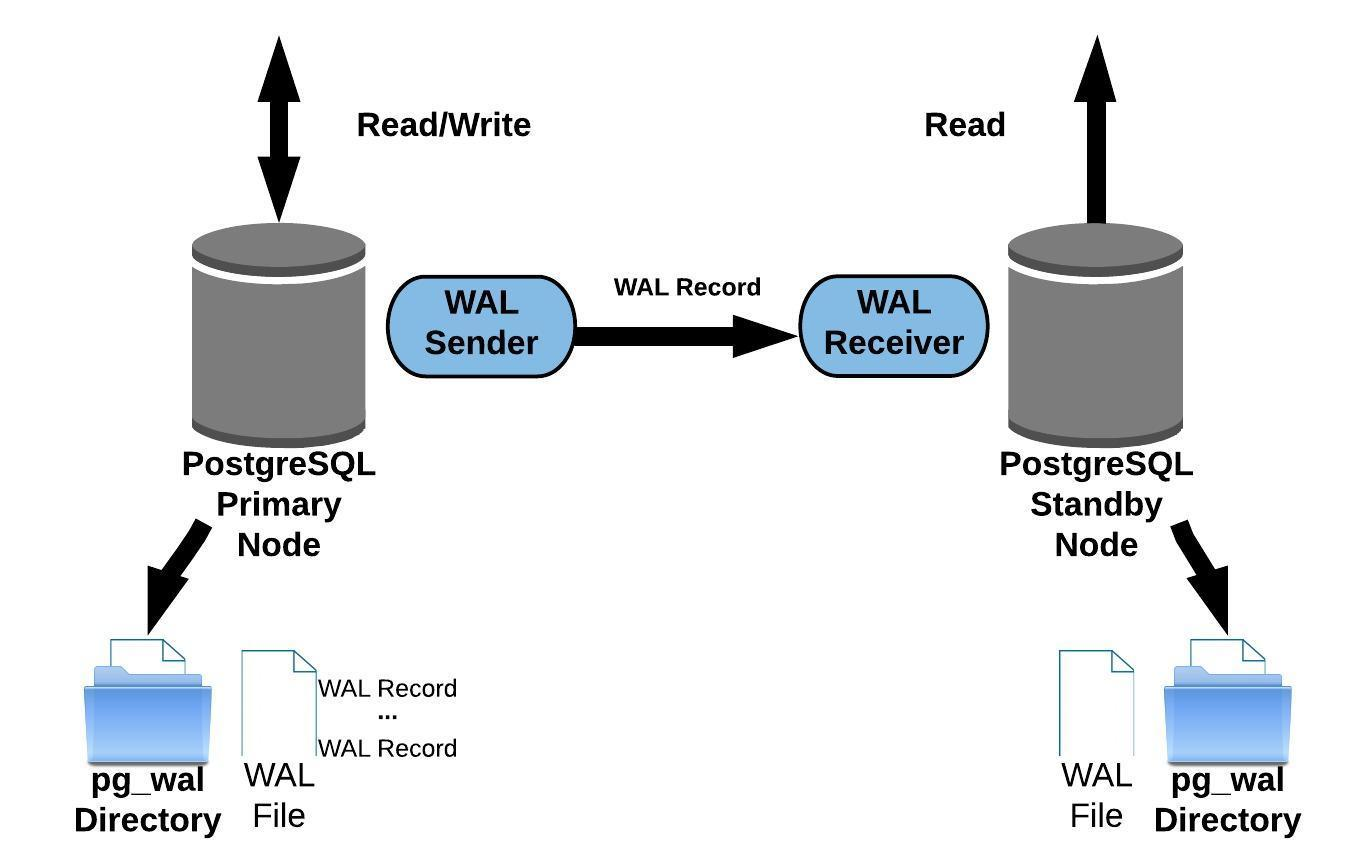
\includegraphics[width=0.75\textwidth,height=\textheight,keepaspectratio]{img/streaming_replication.jpg}
\caption{Streaming Replication di Postgres\\Fonte: \url{https://severalnines.com}}
\label{fig:streaming-replication}
\end{figure}

La replica in streaming può essere costruita in una configurazione 1:N, con un solo server primario, ma è possibile anche aggiungere più server di replica (configurazione \textit{multi-standby}). È anche possibile realizzare una configurazione \textit{a cascata}, in cui un server di replica si connette ad un altro server di replica.

Per la replica in streaming, è possibile scegliere se effettuare una modalità \textit{sincrona} oppure \textit{asincrona}. La differenza tra replica sincrona e replica asincrona sta nell'attesa o meno della risposta dalla replica prima di completare l'elaborazione sul server primario. In particolare:
\begin{itemize}
  \item \textbf{Replica sincrona}: il server primario attende una risposta dal server di replica prima di completare un processo. In questo caso il tempo di risposta complessivo include anche il tempo di spedizione del registro WAL;
  \item \textbf{Replica asincrona} (impostazione predefinita): il server primario completa un processo senza attendere una risposta dal server di standby. Pertanto, il tempo di risposta complessivo è praticamente lo stesso di quando non viene utilizzata la replica in streaming; in questa modalità il risultato aggiornato sul server primario potrebbe non essere immediatamente disponibile sul server di replica. \cite{streaming_replication}
\end{itemize}

Ci sono tuttavia alcune limitazioni nell'utilizzo di repliche con Postgres:
\begin{itemize}
  \item Ogni replica è di sola lettura. Non è possibile creare una replica che sia anche scrivibile;
  \item Non è possibile creare una replica di lettura da un'altra replica di lettura a cascata;
  \item Gli utenti e i ruoli di accesso vengono rispecchiati dall'istanza primaria, il che significa che non è possibile utilizzare credenziali diverse o aggiungere utenti soltanto alla replica;
  \item Non è possibile creare tabelle e viste nell'istanza di replica; in pratica si possono solo eseguire query di tipo \textit{SELECT}.
\end{itemize}

La sezioni seguenti spiegano il lavoro svolto per configurare la replica del database di produzione della piattaforma AirQino.

\subsubsection{Preparazione del database primario}

\begin{enumerate}
  \item Per avviare la procedura, è stato aggiunto sul database un utente Postgres, con un ruolo adatto ad avviare la \textit{streaming replication}, con i comandi SQL:
  \vspace{1mm}
   \begin{lstlisting}[language=sql]
SET password_encryption = 'scram-sha-256'; 
CREATE ROLE repuser WITH REPLICATION PASSWORD 'SOME_SECURE_PASSWORD' LOGIN;\end{lstlisting}
Dove \textit{repuser} è il nome dell'utente di replicazione e\\ \textit{SOME\_SECURE\_PASSWORD} è la password di replicazione;
  \item Sono stati aggiunti i seguenti parametri di configurazione al file \url{/var/lib/postgresql/data/postgresql.conf}:
  \vspace{1mm}
  \begin{lstlisting}[]
listen_addresses= '*'
wal_level = replica
max_wal_senders = 2
max_replication_slots = 2
synchronous_commit = off
\end{lstlisting}
Questi sono i parametri adatti ad una configurazione a replica singola: in caso di più repliche sarà necessario aumentare il valore di \url{max_wal_senders} e \url{max_replication_slots} \cite{stre_re};

  \item Sono stati aggiunti i seguenti parametri al file \url{/var/lib/postgresql/data/pg_hba.conf} per configurare l'autenticazione basata su host, in modo da accettare connessioni dalla replica:
  \vspace{1mm}
\begin{lstlisting}[]
host     replication     repuser   <REPLICA_IP>/32       scram-sha-256
\end{lstlisting}
Dove \textit{repuser} è l'utente creato al passo 1 e \textit{REPLICA\_IP} è l'IP della macchina in cui si trova la replica \cite{stre_re};
  \item È stato riavviato il database per applicare i cambiamenti;
  \item Infine è stato creato uno \textit{slot di replicazione} sul database con il comando:
  \vspace{1mm}
  \begin{lstlisting}[language=sql]
SELECT * FROM pg_create_physical_replication_slot('replica_1_slot');
\end{lstlisting}
Questo assicura che il server master conservi i registri WAL necessari per le repliche anche quando queste sono disconnesse dal master.
\end{enumerate}

\subsubsection{Configurazione della replica}\label{conf-repl}
Di seguito sono elencati i passi eseguiti per configurare e attivare la replica su un server secondario:

\begin{enumerate}
  \item È stata interrotta l'istanza Postgres (se attiva) con il comando:
  \vspace{1mm}
\begin{lstlisting}[]
pg_ctl -D $PGDATA -m fast -w stop
\end{lstlisting}
  \item Sono stati cancellati i contenuti della cartella \textit{PGDATA}:
  \vspace{1mm}
\begin{lstlisting}[]
rm -rf $PGDATA/*
\end{lstlisting}
  \item È stato avviato il backup del database primario:
  \vspace{1mm}
\begin{lstlisting}[]
pg_basebackup -h <PRIMARY_HOST> -p <PRIMARY_PORT> -D $PGDATA -U repuser -vP -R -W
\end{lstlisting}
Dove \textit{PRIMARY\_HOST} è l'IP della macchina in cui si trova il database primario, \textit{PRIMARY\_PORT} è la porta del database primario e \textit{repuser} è l'utente di replicazione creato al passo 1.

Da notare che con la \textit{flag} \textit{-W} viene chiesta in maniera interattiva la password di replicazione, anch'essa impostata in precedenza al passo 1;
  \item Infine è stata riavviata l'istanza Postgres:
  \vspace{1mm}
\begin{lstlisting}[]
pg_ctl -D $PGDATA -w start
\end{lstlisting}
A questo punto la replica è attiva e sincronizzata 1:1 in tempo reale con il database primario. Per il database di produzione AirQino, questa procedura ha richiesto circa 5 minuti.
\end{enumerate}

\subsubsection{Automazione con Docker}
L'intero setup è stato poi automatizzato con Docker \cite{docker} e docker-compose, in modo da avviare la sincronizzazione direttamente all'avvio del container, rendendo la procedura molto più semplice da gestire.

Poichè la creazione della replica richiede l'interruzione dell'istanza Postgres, questa procedura non si può eseguire all'interno del container Docker stesso, perchè si andrebbe a interrompere tutto il container.
Per questo è stato necessario aggiungere i comandi per la replica in uno script di \textit{entrypoint}, che viene eseguito subito prima di avviare il container \cite{dockerfile}:
\begin{enumerate}
  \item È stato creato un \url{Dockerfile} partendo dall'immagine Timescale ufficiale (\url{timescaledb:latest}), con l'aggiunta di uno script \textit{entrypoint}, in questo modo:
  \vspace{1mm}
  \begin{lstlisting}[]
FROM timescale/timescaledb:latest-pg13
ADD replica.sh /docker-entrypoint-initdb.d/
\end{lstlisting}
Dove \url{docker-entrypoint-initdb.d} è una cartella speciale messa che serve proprio a garantire l'esecuzione di qualsiasi file si trovi al suo interno al momento dell'avvio del database;
  \item È stato creato il file \url{replica.sh}, eseguito tutte le volte che si avvia il database, con il seguente contenuto:
  \vspace{1mm}
  \begin{lstlisting}[]
echo "Stopping Postgres instance..." 
pg_ctl -D ${PGDATA} -m fast -w stop

echo "Clearing PGDATA folder..." 
rm -rf ${PGDATA}

echo "Creating base backup..." 
PGPASSWORD=${REPLICATION_PASSWORD} pg_basebackup -h ${REPLICATION_HOST} -p ${REPLICATION_PORT} -D ${PGDATA} -U ${REPLICATION_USER} -vP -R -w

echo "Restarting Postgres instance..." 
pg_ctl -D ${PGDATA} -w start
\end{lstlisting}
Il file riproduce semplicemente i passi descritti in \ref{conf-repl}.

Come già accennato, la flag \textit{-W} di \url{pg\_basebackup} chiede la password in maniera interattiva, ma questo ovviamente non è adatto a script automatizzati che invece non richiedono interazione. Come alternativa è stata utilizzata la flag \textit{-w} (minuscola) e passata la password come una variabile di ambiente (\textit{PGPASSWORD});
\item È stato creato il file \url{docker-compose.yml} così strutturato (ridotto per semplicità):
\vspace{1mm}
  \begin{lstlisting}[]
services:
  replica:
    build:
        context: .
        dockerfile: Dockerfile
    environment:
        PGDATA: /var/lib/postgresql/data/pgdata

        # Parametri di replicazione
        REPLICA_USER: repuser # Utente di replicazione impostato al punto 1
        REPLICATION_HOST: x.x.x.x # IP del db primario
        REPLICATION_PORT: x # Porta del db primario
        REPLICATION_PASSWORD: SOME_SECURE_PASSWORD # Password di replicazione impostata al punto 1
    ports:
        - 45432:5432
    volumes:
        - /var/replica-pg13-timescale/:/var/lib/postgresql/data
\end{lstlisting}
Questo file semplicemente costruisce il container leggendo le istruzioni dal \url{Dockerfile} del passo 1, e applicando le varabili di ambiente specificate nel campo \url{environment}. Ulteriori parametri possono essere specificati, come ad esempio la porta sulla quale viene esposto il database (campo \url{ports}) e la cartella dell'host che viene mappata come volume di dati nel container (campo \url{volumes});
  \item Infine, è stato avviato il container con \url{docker-compose} \url{up}.
\end{enumerate}

In questo modo la replica viene sincronizzata con il database primario automaticamente all'avvio del container Docker (figura \ref{fig:replication}).

\begin{figure}[H]
\centering
\captionsetup{justification=centering}
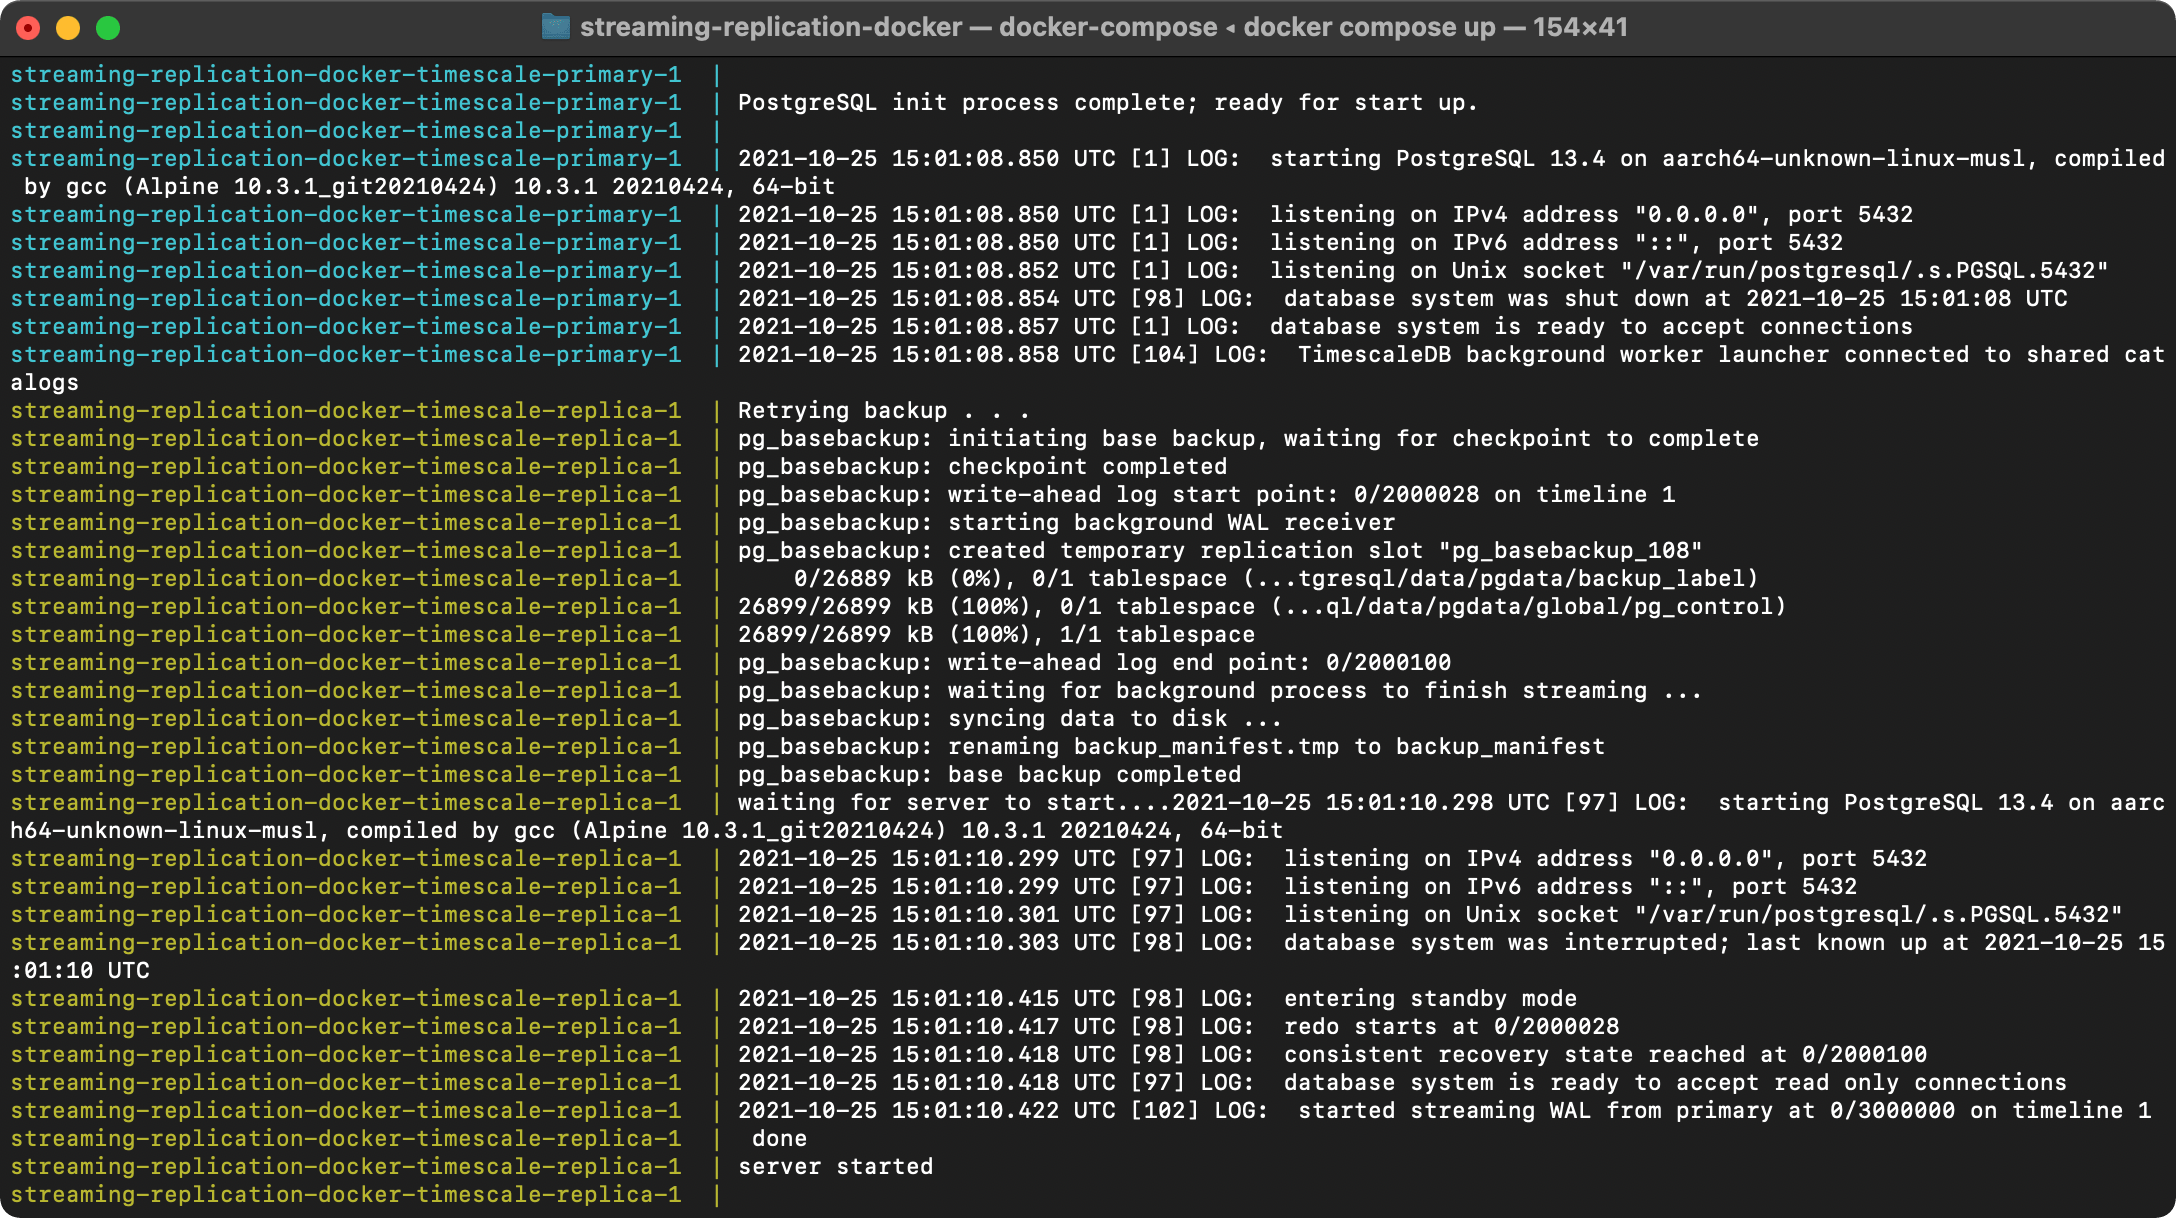
\includegraphics[width=0.75\textwidth,height=\textheight,keepaspectratio]{img/replication}

\caption{Output del comando \url{docker-compose} \url{up} con sincronizzazione automatica della replica del database primario}
\label{fig:replication}
\end{figure}

% Ottimizzazione di query temporali
\section{Ottimizzazione di query temporali}\label{sec:cont-aggr}
Esistono molti vantaggi nell'aggregazione di grandi quantità di dati:
\begin{itemize}
  \item \textbf{Flessibilità}: aggregare dati in tempo reale in base a qualsiasi criterio desiderato;
  \item \textbf{Risparmio di tempo}: non è necessario eseguire query aggiuntive per ottenere altre informazioni;
  \item \textbf{Risparmio di spazio}: i dati aggregati in tempo reale occupano meno spazio rispetto ai dati non aggregati.
\end{itemize}

I dati delle serie temporali (es. misurazioni sensori) tendono a crescere molto rapidamente, e questo può influire sull'esecuzione di query con lo scopo di aggregare i dati (ad esempio per generare report o riepiloghi sull'andamento o sui trend di crescita/decrescita). Per garantire efficienza e scalabilità con questa tipologia di dati, è necessario che le query di aggregazione su dati temporali abbiano un tempo di risposta costante, indipendentemente dalla quantità di dati e senza gravare in maniera eccessiva sul database.

\subsection{Motivazioni}\label{ssec:cont-aggr-motivazioni}
La piattaforma AirQino (vedi \ref{sec:airqino}) raccoglie dati emessi ogni minuto da decine di centraline in diverse località. Per memorizzare questi dati viene utilizzato un database Postgres \cite{postgres} con estensione Timescale \cite{timescale}, che offre delle funzionalità specifiche proprio per dati di tipo temporale.

Una delle funzionalità della piattaforma AirQino consente di mostrare un grafico dell'andamento (su base media oraria) dell'ultima settimana per diverse grandezze (temperatura, umidità, \ce{CO2}, \ce{NO2}, \ce{PM_{2.5}}, \ce{PM_10} etc...), come mostrato in figura \ref{fig:airqino-temp}.

\begin{figure}[H]
\centering
\captionsetup{justification=centering}
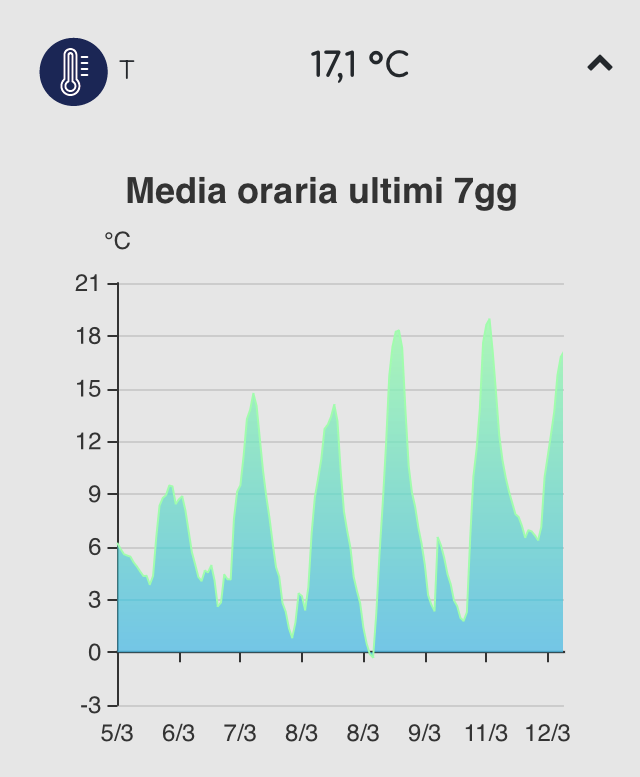
\includegraphics[width=0.45\textwidth,height=\textheight,keepaspectratio]{img/airqino_temp}
\caption{Grafico dell'andamento della temperatura nell'ultima settimana per una centralina AirQino.\\Fonte: \url{https://airqino.magentalab.it}}
\label{fig:airqino-temp}
\end{figure}

La piattaforma prevede inoltre altri casi d’uso per i dati a media oraria:
\begin{itemize}
  \item Visualizzazione sulla home page dell’applicazione le medie orarie degli ultimi 7 giorni;
  \item Esportazione dataset periodici, da mettere a disposizione degli utenti esterni (ad esempio pubbliche amministrazioni che hanno installato le centraline);
  \item Esportazione dataset \textit{on demand} da parte di utenti esterni, con indicazione di inizio/fine del periodo desiderato.
\end{itemize}
In tutti questi casi il requisito è di ottenere \textbf{medie orarie del dato calibrato}.

Per calcolare la media oraria nell'ultima settimana, ad ogni richiesta sul database viene eseguito una query SQL di questo tipo (ridotta per semplicità):

\vspace{1mm}
\begin{lstlisting}[language=sql]
SELECT time_bucket('1 hour', sd.data_acquired) as bucket, avg(sd.float_value)
FROM station_data sd
WHERE sd.data_acquired > NOW() - INTERVAL '7 days'
AND sd.sensor_id = 29510691 /* id centralina */
ORDER BY bucket DESC;
\end{lstlisting}

Dove \textit{station\_data} è la tabella contenente i dati dei sensori, la colonna \textit{data\_acquired} rappresenta data e ora di misurazione e la colonna \textit{float\_value} indica il valore grezzo della misurazione.
I dati vengono limitati solo all'ultima settimana tramite una comparazione su clausola \textit{WHERE}.

La query inoltre fa uso della funzione \textit{time\_bucket} di Timescale, che consente di partizionare la tabella con i dati dei sensori minuto per minuto direttamente in fasce orarie; l'utilizzo combinato con la funzione \textit{avg()} consente poi di estrarre la media del valore su tutta l'ora.

Questo però significa che se si desidera eseguire questa query più di una volta, il database deve eseguire la scansione dell'intera tabella e ricalcolare la media ogni volta. Questo risulta poco efficiente, perchè nella maggior parte dei casi i dati nella tabella non sono cambiati in modo significativo, quindi non è necessario eseguirne nuovamente la scansione.

La figura \ref{fig:query-prima} mostra i tempi di risposta della query per estrarre la media oraria di \ce{NO2} per tutte le centraline AirQino, prima di aver applicato l'ottimizzazione.

\begin{figure}[H]
\centering
\captionsetup{justification=centering}
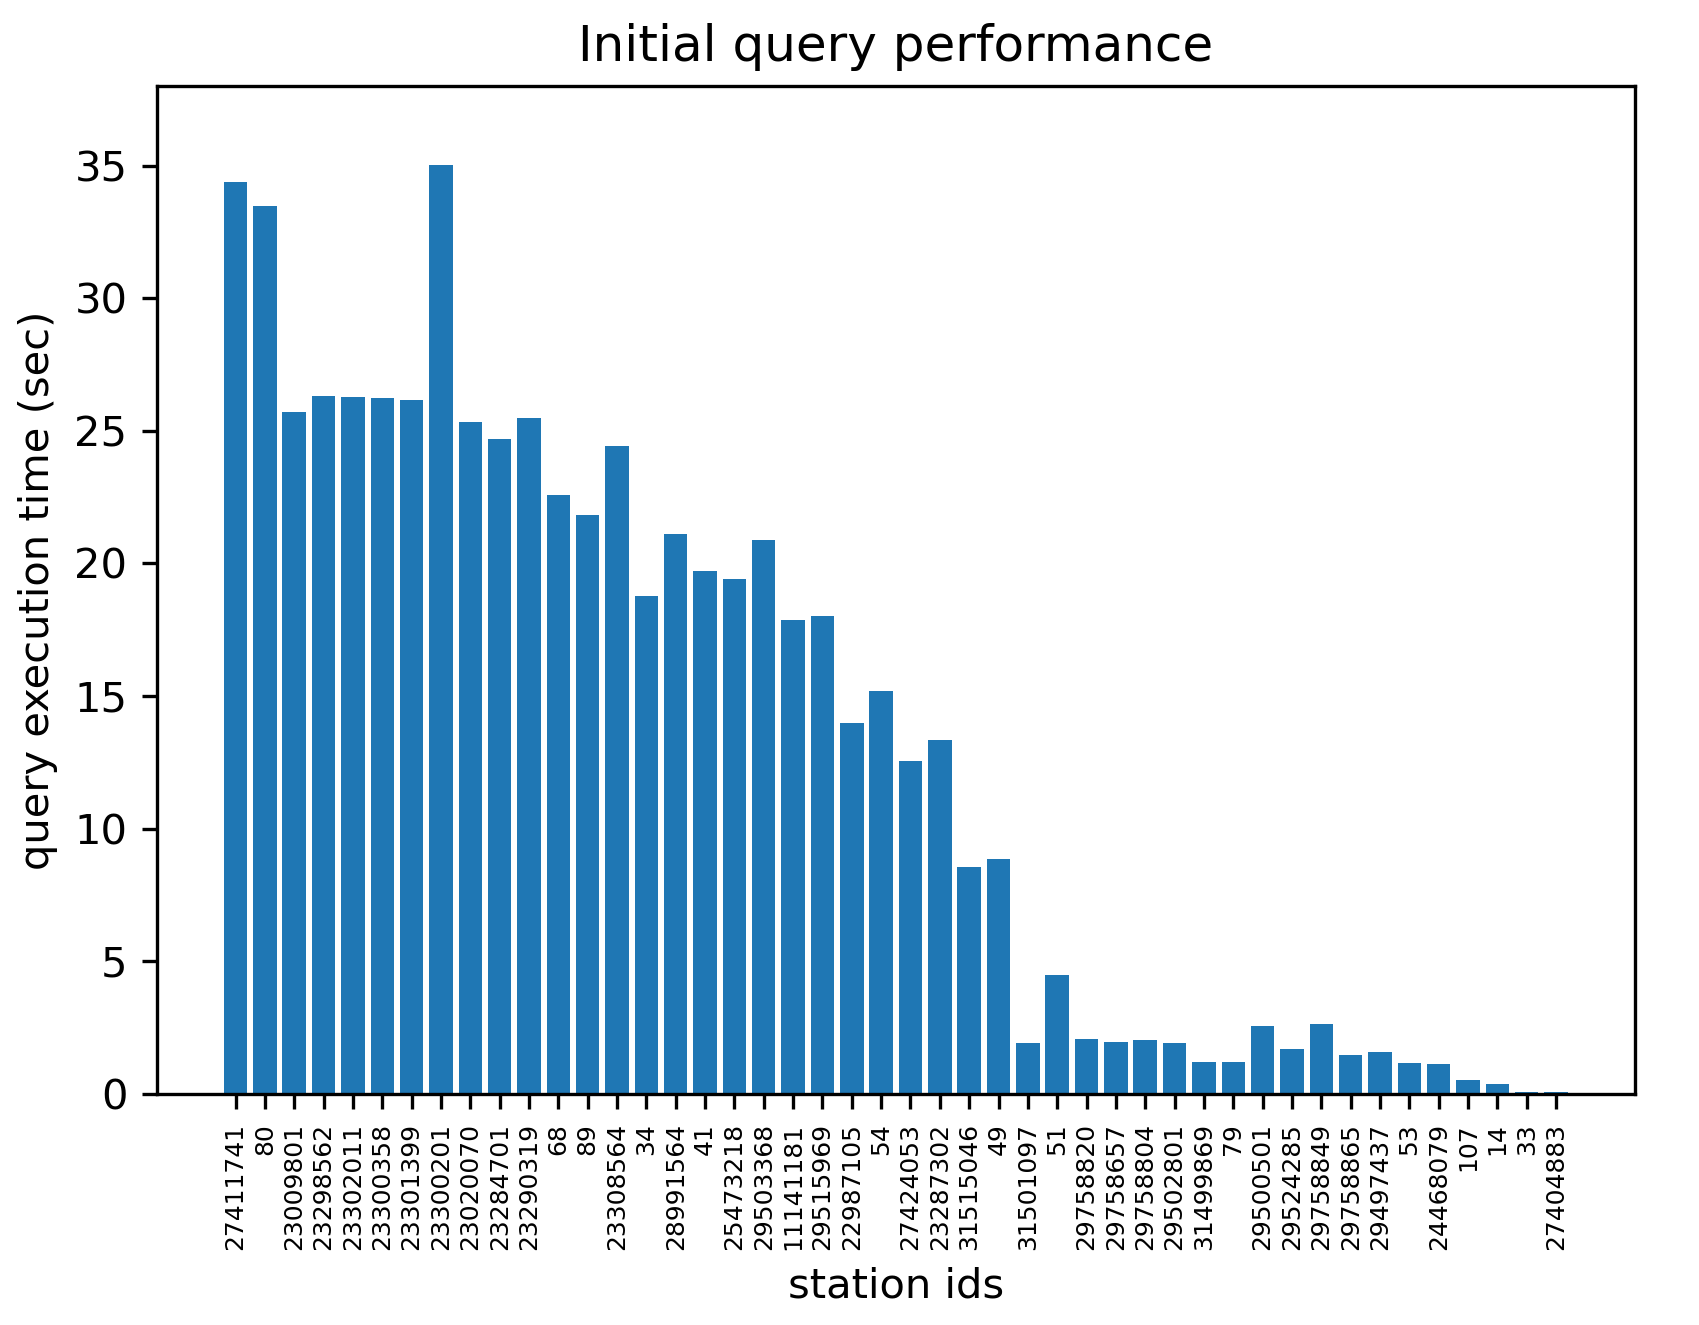
\includegraphics[width=0.85\textwidth,height=\textheight,keepaspectratio]{img/query_prima}
\caption{Tempi di risposta della query per estrarre la media oraria di \ce{NO2} dell'ultima settimana per tutte le centraline AirQino, prima dell'ottimizzazione (media su 10 iterazioni)}
\label{fig:query-prima}
\end{figure}

Come si può vedere, la query per recuperare la media oraria impiega fino a 35 secondi per le centraline più attive, un tempo molto elevato.

Per affrontare questo tipo di problema e rendere più veloce l'aggregazione dei dati, Timescale mette a disposizione una funzionalità chiamata \textbf{continuous aggregates} (\textit{aggregati continui}).

\subsection{Continuous aggregates}\label{ssec:cont-aggr}
I continuous aggregates sono una funzionalità integrata in Timescale che consente di aggregare i dati in tempo reale, senza la necessità di eseguire query aggiuntive \cite{timescale_ca_2}. Il funzionamento è simile alle \textbf{viste materializzate} di Postgres, con la differenza che i continuous aggregates non necessitano di essere aggiornati manualmente ogni volta che un nuovo dato viene inserito nella tabella. Infatti, la riaggregazione viene eseguita automaticamente in background tramite una \textbf{refresh policy} definita dall'utente in fase di creazione della vista.

L’utilizzo dei countinuous aggregates offre diversi vantaggi:
\begin{itemize}
  \item Miglioramento delle \textbf{performance}, infatti non è più necessario scansionare tutte le volte la tabella con i dati raw ma è sufficiente leggere questi risultati precalcolati;
  \item Funzionalità avanzate, come la possibilità di salvare i dati raw solo per un periodo di tempo limitato, continuando però a mantenere i dati aggregati. Così facendo si hanno dei dati riassuntivi per eventi che sono molto indietro nel tempo, mentre per gli eventi più recenti si continua ad avere tutti i dati raccolti, portando and un grosso \textbf{risparmio di spazio occupato}. \cite{tesi_polito_2}
\end{itemize}

Di contro, lo svantaggio di questa soluzione è che i dati non sono aggiornati ad ogni INSERT effettuata, ma solo ad un intervallo di tempo specificato dall’utente. Questo significa che in fase di lettura i dati più recenti non sono presenti nelle viste materializzate. Per limitare questo problema si potrebbe pensare di diminuire l’intervallo di tempo necessario per il refresh dei dati, ma questo porterebbe ad un aumento del carico computazionale. C'è quindi un compromesso tra la velocità di lettura e l’aggiornamento dei dati. \cite{tesi_polito_2}

Timescale inoltre introduce il concetto di \textit{hypertable}, normali tabelle SQL ma con partizionamento automatico su base temporale.

\subsection{Risultati ottenuti}\label{ssec:cont-aggr-risultati}
Di seguito sono riportati i passi eseguiti sul database di produzione AirQino per l'attivazione del meccanismo di continuous aggregates sulla tabella con i dati dei sensori (\textit{station\_data}):

\begin{enumerate}
  \item È stata creata la \textit{hypertable} a partire dalla tabella originale, avendo cura di migrare tutti i dati (questo è necessario perchè i continuous aggregates si applicano solo alle \textit{hypertable}):
\vspace{1mm}
\begin{lstlisting}[language=sql]
SELECT create_hypertable('station_data', 'data_acquired', migrate_data => true);
\end{lstlisting}
Dove \textit{data\_acquired} è la colonna temporale della tabella, in cui vengono salvati data e ora della misurazione.
Questa operazione potrebbe impiegare molto tempo in base alla quantità di dati nella tabella; sul database di produzione AirQino ha richiesto circa 36 minuti;
  \item È stata creata la vista materializzata per il calcolo delle medie orarie con continuous aggregates:
\vspace{1mm}
\begin{lstlisting}[language=sql]
CREATE MATERIALIZED VIEW station_data_hourly_avg
WITH (timescaledb.continuous) AS
SELECT time_bucket('1 hour', sd.data_acquired) AS bucket, 
    station_id,  
    sensor_id, 
    avg(sd.float_value) 
FROM station_data sd
GROUP by bucket, station_id, sensor_id;
\end{lstlisting}
Dove il nome dell'aggregato è \textit{station\_data\_hourly\_avg}, mentre la funzionalità di aggregazione continua viene specificata nella clausola \textit{WITH}. Nella \textit{SELECT} invece sono stati specificati la tabella di partenza (\textit{station\_data}), l'intervallo di aggregazione (\textit{1 hour}) e l'operazione da eseguire per aggregare i dati (\textit{avg()}, ovvero la media).
Questa operazione sul database di produzione AirQino ha richiesto circa 5 minuti;
  \item Infine, è stata creata una \textit{refresh policy} adeguata con il comando:
\vspace{1mm}
\begin{lstlisting}[language=sql]
SELECT add_continuous_aggregate_policy('station_data_hourly_avg',
     start_offset => INTERVAL '7 days',
     end_offset => INTERVAL '1 hour',
     schedule_interval => INTERVAL '1 hour');
\end{lstlisting}
Dove \textit{start\_offset} indica quanto indietro nel tempo si va a calcolare l'aggregato, \textit{end\_offset} indica fino a quando fermarsi e \textit{schedule\_interval} indica l'intervallo di aggiornamento della lista.
In questo caso è stato scelto di aggiornare, ogni ora, i dati della settimana passata, fino a un'ora prima del tempo di esecuzione.
Per ragioni di performance conviene sempre escludere l'ultimo \textit{bucket} (in questo caso l'ultima ora di dati arrivati). \cite{timescale_ca}
\end{enumerate}

Una volta creata la vista, è possibile riscrivere la SELECT originale per la media degli ultimi 7 giorni, ma stavolta prendendo i dati da questa nuova tabella con aggregati continui (\textit{station\_data\_hourly\_avg}):
\vspace{1mm}
\begin{lstlisting}[language=sql]
SELECT sd.avg
FROM station_data_hourly_avg sd
WHERE bucket > NOW() - INTERVAL '7 days'
AND sd.sensor_id = 29510691 /* id centralina */
ORDER BY bucket DESC;
\end{lstlisting}

Questa query è risultata molto più performante rispetto alla precedente, essendo le medie orarie di fatto già precalcolate e sempre aggiornate in background. I nuovi risultati sulle centraline AirQino sono riportati di seguito in figura \ref{fig:query-dopo}.

\begin{figure}[H]
\centering
\captionsetup{justification=centering}
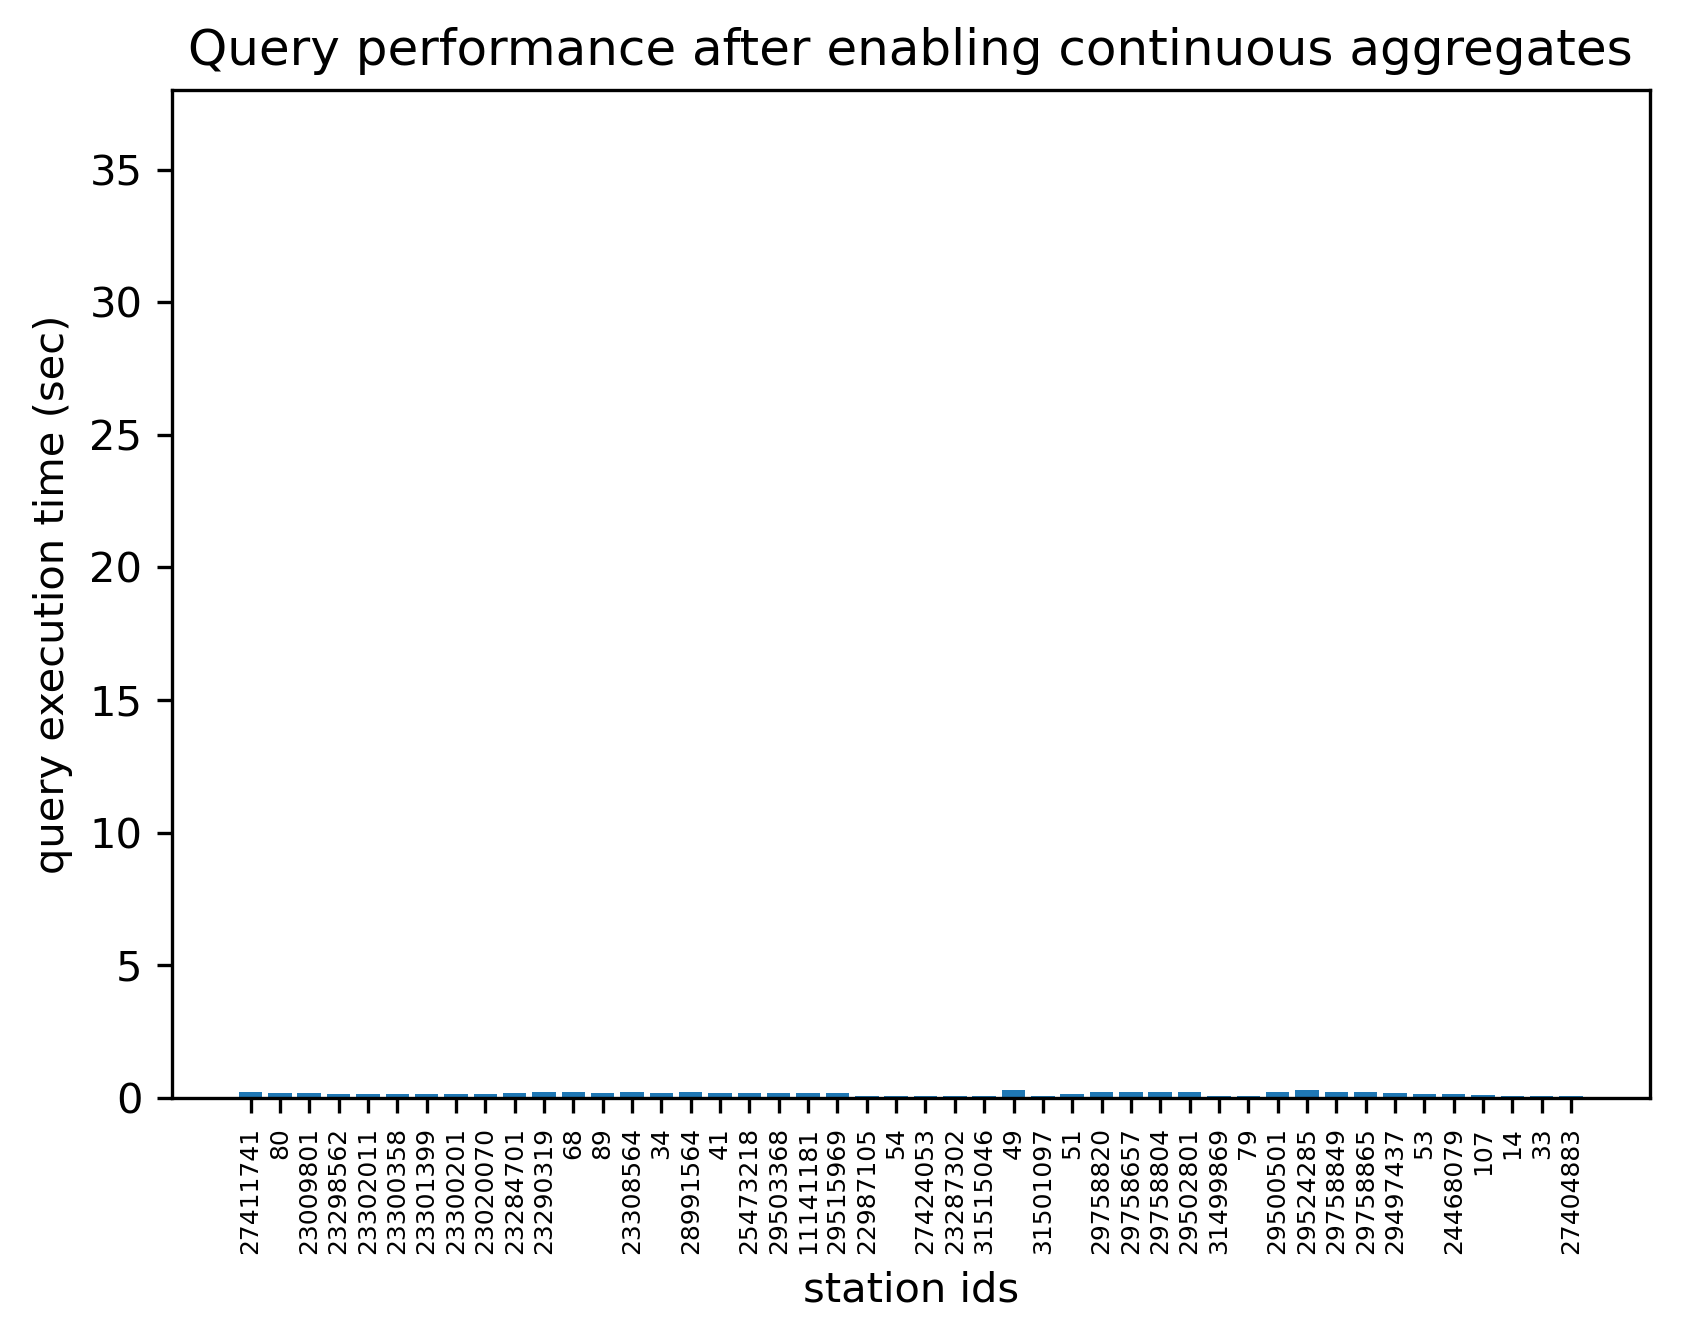
\includegraphics[width=0.85\textwidth,height=\textheight,keepaspectratio]{img/query_dopo}
\caption{Tempi di risposta della query per estrarre la media oraria di \ce{NO2} dell'ultima settimana per tutte le centraline AirQino, dopo l'ottimizzazione (media su 10 iterazioni)}
\label{fig:query-dopo}
\end{figure}

Da cui si può notare che con la nuova query, ottimizzata con continuous aggregates, i tempi di risposta risultano costanti per tutte le centraline, indipendentemente dalla quantità di dati (con conseguente riduzione significativa dei tempi di risposta, anche 175 volte meno per alcune centraline), garantendo maggiore \textbf{scalabilità} ed \textbf{efficienza} al sistema.
